\documentclass[12pt]{article}
\usepackage{amsmath}
\usepackage{latexsym}
\usepackage{amsfonts}
\usepackage{amssymb}
\usepackage{graphicx}
\usepackage{txfonts}
\usepackage{wasysym}
\usepackage{adjustbox}
\usepackage{ragged2e}
\usepackage{tabularx}
\usepackage{hhline}
\usepackage{float}
\usepackage{multirow}
\usepackage{makecell}
\usepackage{fancyhdr}
\usepackage[utf8]{inputenc}
\usepackage[T1]{fontenc}
\usepackage[a4paper,bindingoffset=0.2in,headsep=0.5cm,left=1in,right=1in,bottom=3cm,top=2cm,headheight=2cm]{geometry}
\usepackage{hyperref}
\usepackage{listings}

\everymath{\displaystyle}
\pagestyle{fancy}
\fancyhf{}
\rfoot{Page \thepage}
\begin{document}
\sloppy 

\begin{center}
\Large Telecom ParisTech \\
\Large COMELEC Department \\
\vspace{20 pt}
\underline{\Huge Development Infrastructure for TTool}
\end{center}

\begin{table}[H]
\large
\centering
\begin{adjustbox}{width=\textwidth}
\begin{tabular}{ |p{1.6cm}|p{6.0cm}|p{4.2cm}|p{4.2cm}| }
\hhline{----}
 & \textbf{Document Manager} & \textbf{Contributors}  & \textbf{Checked by}  \\ 
\hhline{----}
\textbf{Name}   & Dominique BLOUIN & \multirow{2}{*}{Ludovic APVRILLE} &
\multirow{2}{*}{Ludovic APVRILLE} \\
\hhline{--~~}
\textbf{Contact} & dominique.blouin@telecom-paristech.fr &  &  \\ 
\hhline{--~~}
\textbf{Date} & \today &  &  \\ 
\hline
\end{tabular}
\end{adjustbox}
\end{table}

\newpage
\tableofcontents

% \newpage
% \listoffigures

\newpage
\section{Preface}

\subsection{Table of Versions}

\begin{table}[H]
\large
\centering
\begin{adjustbox}{width=\textwidth}
\begin{tabular}{ |p{1.5cm}|p{2.5cm}|p{9.0cm}|p{3.0cm}| }
\hhline{----}
\textbf{Version} & \textbf{Date} & \textbf{Description  $  \&  $  Rationale of
Modifications} & \textbf{Sections Modified} \\
\hhline{----}
1.0 & 17/10/2016 & First draft &  \\ 
1.1 & 10/02/2017 & Added Eclipse IDE development + tests & All \\ 
1.2 & 11/02/2017 & Added more info on tests & Tests \\ 
\hline
\end{tabular}
\end{adjustbox}
\end{table}

\subsection{Table of References and Applicable Documents}

\begin{table}[H]
\large
\centering
\begin{adjustbox}{width=\textwidth}
\begin{tabular}{ |p{2.66in}|p{2.66in}|p{0.95in}|p{0.43in}| }
\hhline{----}
\textbf{Reference} & \textbf{Title  $  \&  $  Edition} & \textbf{Author or
Editor} & \textbf{Year}
\\
\hhline{----}
 &  &  &  \\ 
\hline
\end{tabular}
\end{adjustbox}
\end{table}

\subsection{Acronyms and glossary}

\begin{table}[H]
\large
\centering
\begin{adjustbox}{width=\textwidth}
\begin{tabular}{ |p{1.24in}|p{5.45in}| }
\hhline{--}
\textbf{Term} & \textbf{Description} \\ 
\hhline{--}
 &  \\ 
\hline
\end{tabular}
\end{adjustbox}
\end{table}

\subsection{Executive Summary}

This document describes the development infrastructure that has been setup for
the development of TTool. It describes sources configuration management, the
development process with basic editor and command lines, with the Eclipse IDE,
as well as the testing, building and installation procedures.

\section{Source Configuration Management}
\label{sec:scm}

\subsection{Gitlab Server}

TTool sources are hosted on the Gitlab server of Telecom ParisTech under the
group \textit{mbe}\textit{-tools} and project \textit{TTool}. The Gitlab project
can be accessed via . Login must be performed using Shibboleth as shown in
figure~\ref{fig:image1}, using the credentials from your institution if it is a
member of the Federation Education Recherche (\url{https://services.renater.fr/federation/participants/idp}). Otherwise, please ask us for an account.

\begin{figure}[H]
\begin{center}

\includegraphics[width=\textwidth]{images/image1.png}
\end{center}
\caption{}
\label{fig:image1}
\end{figure}
 
\subsection{Basic Sources Management}

The address to access the sources is . For the time being and until further notice, we will keep using a centralized development process, like it was the case for Subversion. In this process, each developer first obtains a clone of the master remote repository. For this, go to the directory where the sources are to be downloaded and issue the following command: \\


\begin{verbatim}
git clone git@gitlab.enst.fr:mbe-tools/TTool.git
\end{verbatim}

Once modifications are made, they can be committed using command:

\begin{verbatim}
git commit -m "Commit message"
\end{verbatim}

This will only commit the changes in your local repository. In order to move them to the remote repository, use:

\begin{verbatim}
git push origin master
\end{verbatim}

More information on the use of Git can be found here: \\
\url{http://rogerdudler.github.io/git-guide/}. \\

By default, Git will ask credentials for each operation. In order to avoid this,
it is possible to upload a public SSH key at: \\
\url{https://gitlab.telecom-paristech.fr/profile/keys}.

\subsection{Bug Tracking}

The Gitlab server provides an issues tracking system to record bugs, evolutions
or support demands from users and developers. Issues can be seen at: \\
\url{https://gitlab.telecom-paristech.fr/mbe-tools/TTool/issues} \\

It is suggested to create an issue for every modification that is made to the
code, providing with the issue detailed information on the problem including
screen shots, log traces and test cases if required. This information is
important so that other developers can understand why the changes were made.
Ideally, the issue number should be mentioned within the modified code and
commit messages.  \\

\section{Development with Text Editor (emacs, vi) and Make}

The text editor of your choice can be used to edit the files of TTool. Yet, you must be sure that the correct indentation is respected. Use \textbf{4 spaces for each indentation level}.\\

Also, don't forget to insert your name at the top of the file in the authors list.\\

The main Makefile can be used to compile the source files of TTool, and to generate the jar libraries in bin/.
To compile TTool, do as follows, from the top directory of TTool:
\begin{verbatim}
$ make all
\end{verbatim}
or:
\begin{verbatim}
$ make
\end{verbatim}

Other compilation targets can be obtained with:
\begin{verbatim}
$ make help
\end{verbatim}
In particular, to compile the sources without generating the \textit{jar} files can be done with the \textit{ttool} target:
  \begin{verbatim}
$ make ttool
\end{verbatim}



\section{Development with Eclipse}

Eclipse is a well-known Integrated Development Environment (IDE) providing many advanced functionalities to support developers and improve code quality by the application of built-in on the fly code analyses. One advantage of Eclipse is that it is a multi-platform application so it can be used on Linux, Windows and Mac. The procedures described in this section are valid for all platforms although some elements such as C++ projects need to be different due to different platform-specific compilation tool chains to be used. More information on this is provided on the concerned subsections. \\

\subsection{Installing and Configuring Eclipse}

Download Eclipse IDE for Java developers here: \\
\url{http://www.eclipse.org/downloads/packages/eclipse-ide-java-developers/neon2}
\\

Unzip the package and launch the eclipse executable. For developing C++
applications such as the DIPLODOCUS simulator, add the C Development Tools
(CDT). For this, select menu ``Help >> Install New Software''.
From the dialog box that opens, select the ``Neon'' update site, unfold the
``Programming Languages'' category and check the elements as shown in
figure~\ref{fig:image2}. Follow the wizard instructions to complete the
installation.

\begin{figure}[H]
\begin{center}
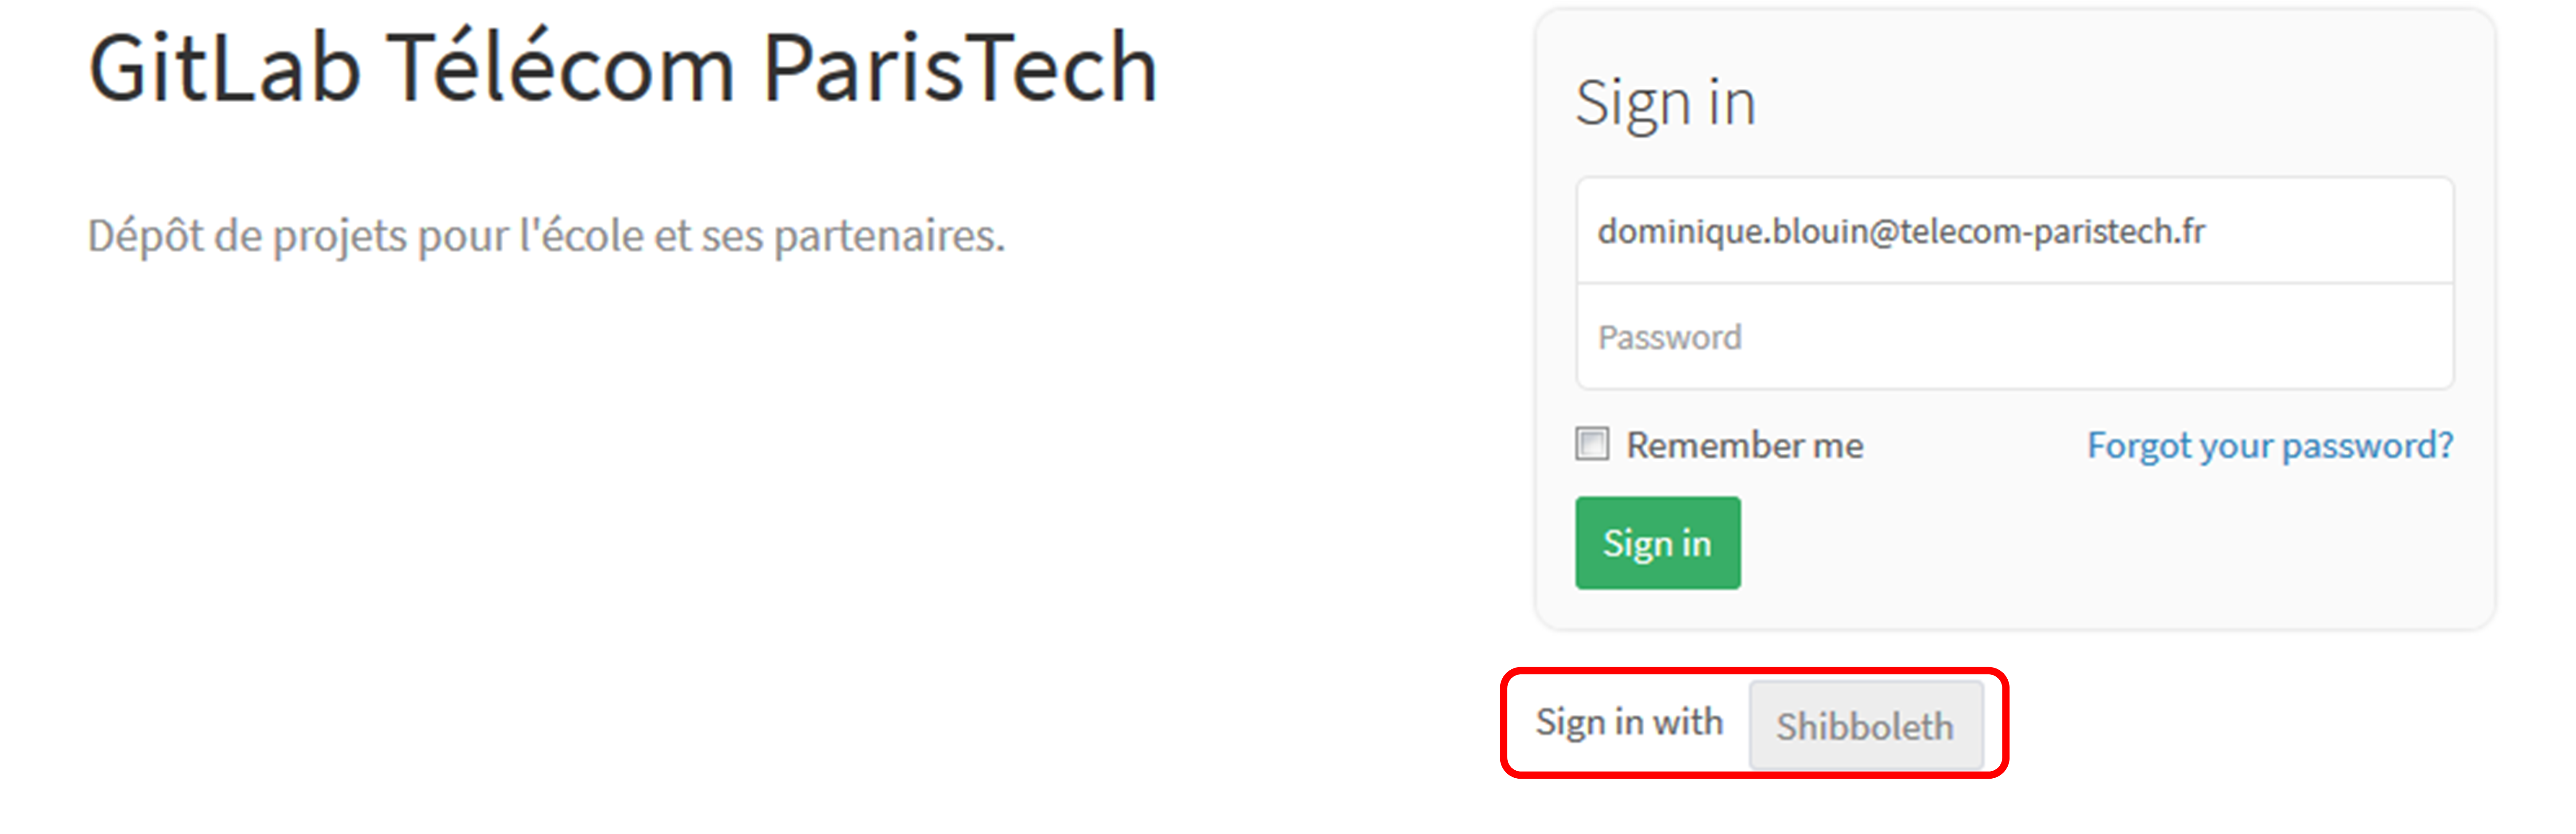
\includegraphics[width=\textwidth]{images/image2.png}
\caption{}
\label{fig:image2}
\end{center}
\end{figure}

\subsection{Online Help}

The first place to look for help is in via menu ``Help>>Help Content'' from
Eclipse. A dialog box will show a tree with branches for each integrated plugin
or application. Help is provided for the 3 plugins that are used to develop
TTool; EGit, Java Development Tools and C/C++ Development Tools.

\subsection{Source Configuration Management with EGit}

The downloaded Eclipse IDE already includes a plugin named EGit for source
configuration management using Git.

\subsubsection{Cloning the TTool Repository}

First, switch to the Git perspective by clicking menu
``Window>>Perspective>>Open Perspective>>Other''. Then select the Git
perspective as illustrated in figure~\ref{fig:image3}.

\begin{figure}[H]
\begin{center}
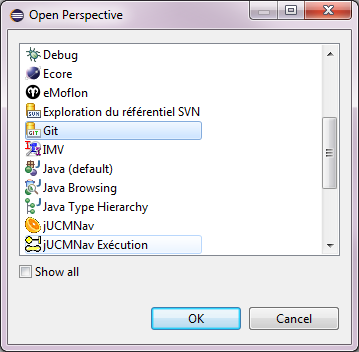
\includegraphics[width=0.6\textwidth]{images/image3.png}
\end{center}
\caption{}
\label{fig:image3}
\end{figure}

Then clone the TTool Git repository by clicking the appropriate button as shown
in figure~\ref{fig:image4}. Specify the TTool Git repository URI
(git@gitlab.enst.fr:mbe-tools/TTool.git) and follow the wizard by also setting
the local Git repository path.

\begin{figure}[H]
\begin{center}
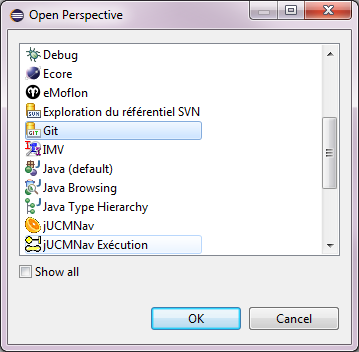
\includegraphics[width=0.6\textwidth]{images/image4.png}
\end{center}
\caption{}
\label{fig:image4}
\end{figure}

The content of the cloned repository can be seen from the Git Repository view by
unfolding the ``Working Tree'' folder (figure~\ref{fig:image5}).

\begin{figure}[H]
\begin{center}
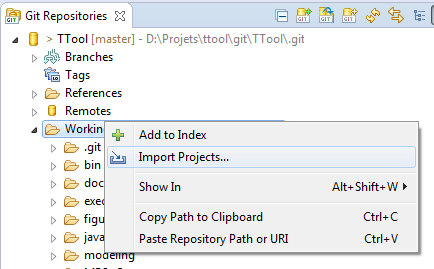
\includegraphics[width=0.6\textwidth]{images/image5.png}
\end{center}
\caption{}
\label{fig:image5}
\end{figure}

\subsubsection{Importing the Required Projects into the Workspace}
\label{sec:import}

Two Eclipse Java projects are needed to develop TTool: the \textit{bin} project
that contains the required libraries (jars) and the \textit{src} project that
contains the source code. Install these 2 projects in the workspace by
right-clicking the ``Working Tree'' it in the Git repository view and
selecting ``Import Projects\ldots'' as shown in figure~\ref{fig:image5}.

Then select ``Import existing Eclipse projects'' as shown in
figure~\ref{fig:image6} and follow the steps of the wizard.

\begin{figure}[H]
\begin{center}
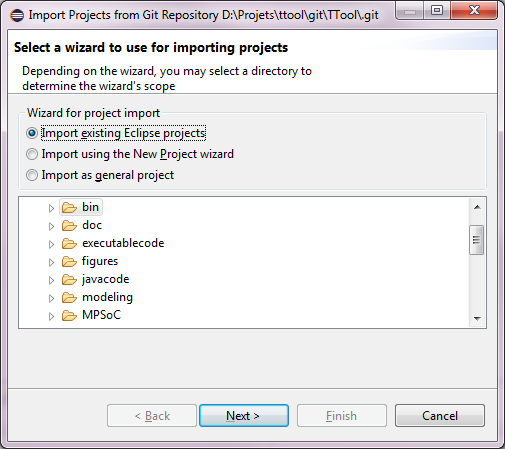
\includegraphics[width=0.7\textwidth]{images/image6.png}
\end{center}
\caption{}
\label{fig:image6}
\end{figure}

\subsubsection{Committing, Pulling and Pushing Changes}

Committing the changes of a file or a directory or a project is performed by
selecting this element in the project navigator view then selecting
``Team>>Commit''. This will open the Git Staging view for where the changed
files are listed. Double clicking a file in the unstaged changes view will open
an editor allowing visualizing the changes (figure~\ref{fig:image7}). Right click and select
``Add to Index'', then enter a commit message and click the ``Commit'' button to
commit the changes. Pushing and pulling can be performed by selecting the repository from
the Git repository view or the elements from the project view.

\begin{figure}[H]
\begin{center}
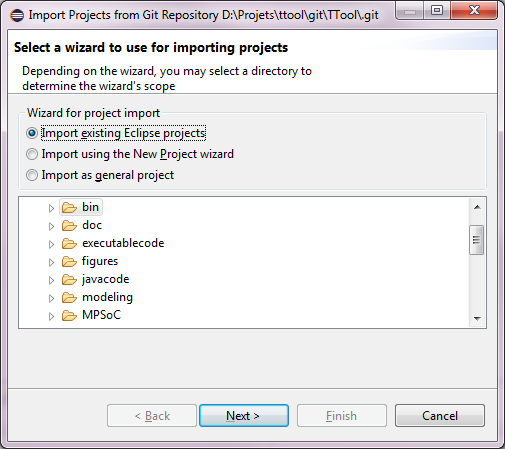
\includegraphics[width=\textwidth]{images/image7.png}
\end{center}
\caption{}
\label{fig:image7}
\end{figure}

\subsection{Java Development}

\subsubsection{Coding and Compiling}

Switch to the Java perspective to develop TTool with JDT (select menu
``Windows>>Perspective\ldots'' or select the appropriate perspective button from
the upper right corner of Eclipse). By default Eclipse will automatically
compile all files in the project. However the provided projects have already
been configured so that only the required classes are compiled and also to use
the required library files from the \textit{bin} project.

JDT provides several advanced functionalities such as automatically navigating
from a variable to its declaration, finding its use throughout all the classes,
including refactoring capabilities, syntactic coloration, code completion, etc.

\subsubsection{Launching TTool}
\label{sec:launch}

A default launch configuration is provided with the TTool \textit{src} project.
It allows for launching TTool from the compiled code. This configuration can be
edited by opening the \textit{Run Configurations} dialog box as show in figure~\ref{fig:image8}.

\begin{figure}[H]
\begin{center}
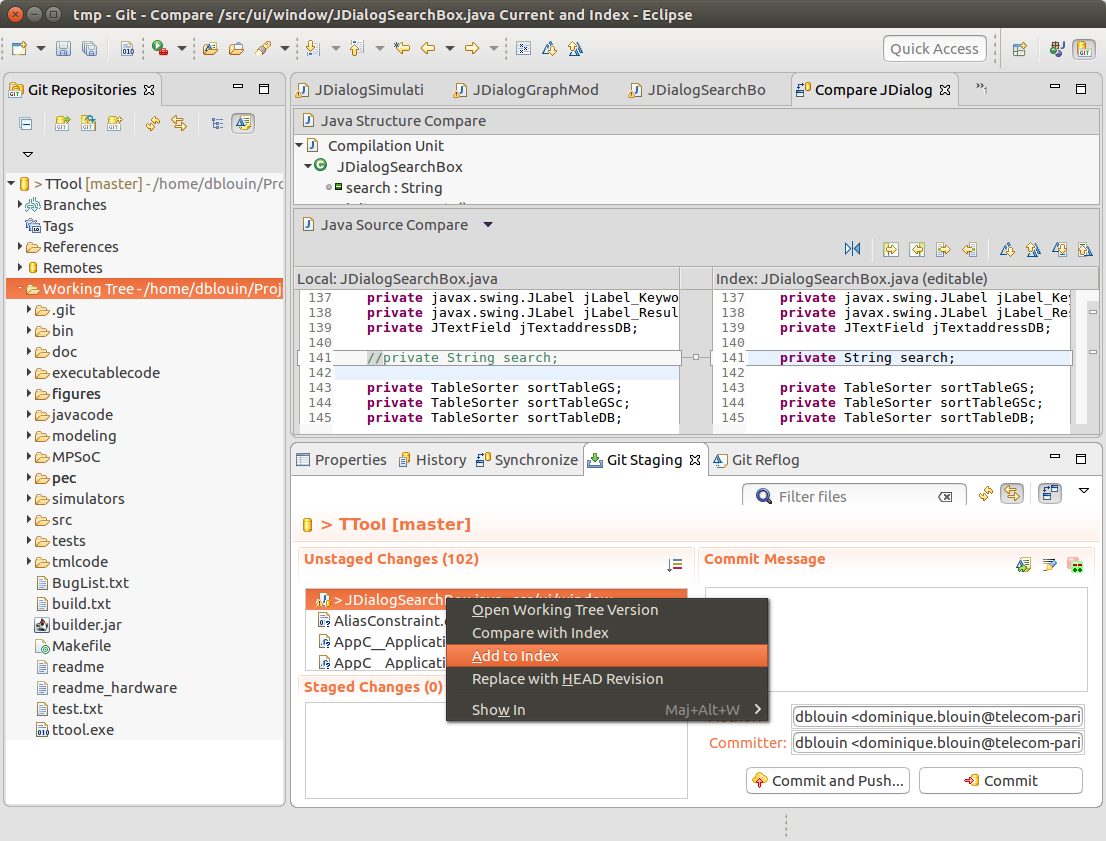
\includegraphics[width=0.9\textwidth]{images/image8.png}
\end{center}
\caption{}
\label{fig:image8}
\end{figure}

The TTool launch configuration is displayed in figure~\ref{fig:image9}. It
specifies the main class to execute as well as the program arguments, working directory and
optionally additional environment variables to be added to the default system
environment. Click \textit{Run} to launch TTool. The output from TTool will be
displayed in the console view. Once TTool has been launched once, simply
clicking the button to open the launch dialog box will directly launch TTool so
that it is not necessary to open the launch dialog box every time.

\begin{figure}[H]
\begin{center}
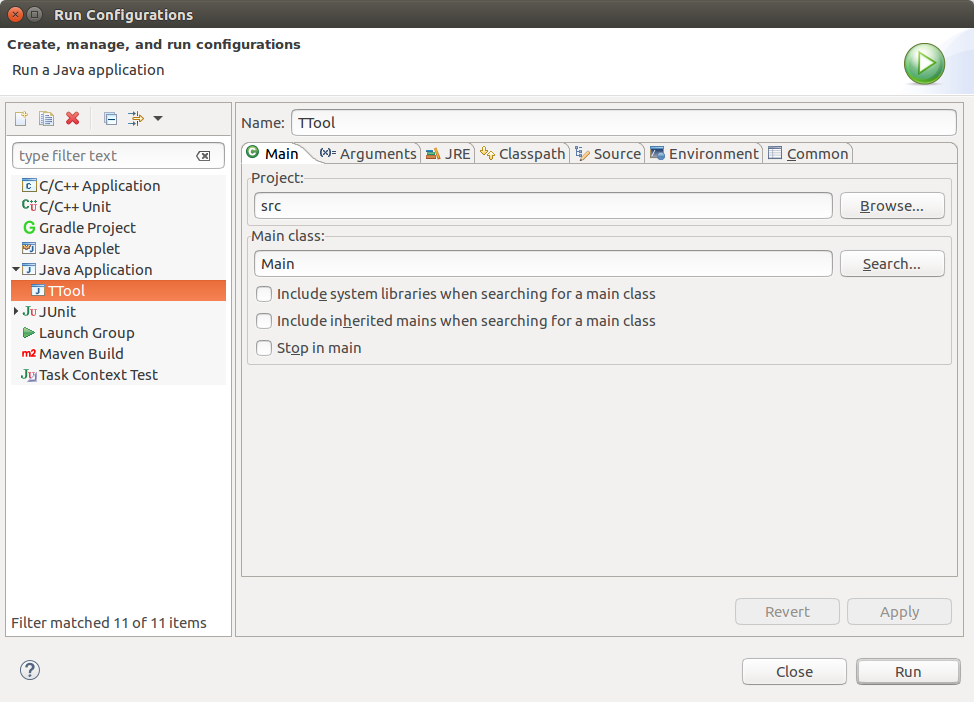
\includegraphics[width=\textwidth]{images/image9.png}
\end{center}
\caption{}
\label{fig:image9}
\end{figure}

\subsubsection{Using the Debugger}

In addition, JDT provides an enhanced debugger allowing executing the program
step by step with sophisticated breakpoints to control the execution and to
examine variable contents etc. However to use the debugger, the proper launch
configurations must be used by clicking the \textit{debug}
button just left of the launch configuration button of figure~\ref{fig:image8}.

\subsection{C++ Development}

One advantage of IDEs is that once a user has learned how to use a first tool,
other integrated tools are faster to learn because the tools share so much
functionality.

\subsubsection{Coding and Compiling}

Like for JDT, CDT also has its own perspective and the first thing to do is to
switch to this perspective as shown in figure~\ref{fig:image10}.

\begin{figure}[H]
\begin{center}
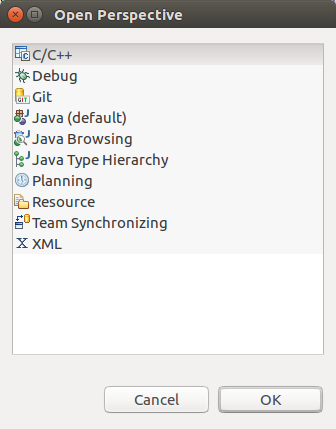
\includegraphics[width=0.45\textwidth]{images/image10.png}
\end{center}
\caption{}
\label{fig:image10}
\end{figure}

For developing the TTool C++ applications with CDT, the predefined CDT projects
must first be imported into the workspace as explained in
section~\ref{sec:import}. Note that for CDT, the projects are platform dependent
due to the different compilation toolchains (Cygwin is used for Windows) so there is one project per
platform. For instance, for developing the DIPLODOCUS simulator on Linux, import
the \textit{c++}\textit{2} project. For windows, import the
\textit{c++}\textit{2 $  \_  $ windows} project (TODO to be provided later). CDT
provides the ability to define several build configurations. For the
\textit{c++}\textit{2} project, two configurations are provided as shown in
figure~\ref{fig:image11}.

\begin{figure}[H]
\begin{center}
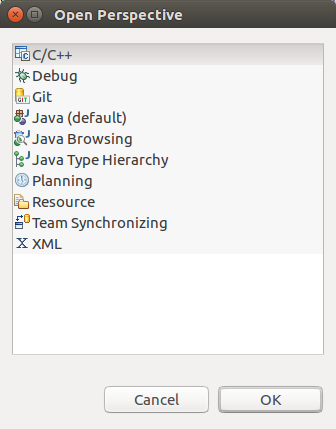
\includegraphics[width=\textwidth]{images/image11.png}
\end{center}
\caption{}
\label{fig:image11}
\end{figure}

The \textit{TTool} configuration will compile the code using the provided make
file as if the simulator were compiled from TTool. The \textit{Debug}
configuration allows for compiling TTool such that it can be executed in debug
mode. The selected button in figure~\ref{fig:image11} allows changing the configuration being
used. The hammer button on the right hand side of it allows compiling and
linking the code.

The settings for these build configurations can be edited by selecting the
\textit{c++2} project in the project navigator and clicking
``Properties''. For the \textit{Debug} configuration, the CDT internal builder
is used. This means that the compilation and linking options can be changed via
the form editor shown in figure~\ref{fig:image12}.

\begin{figure}[H]
\begin{center}
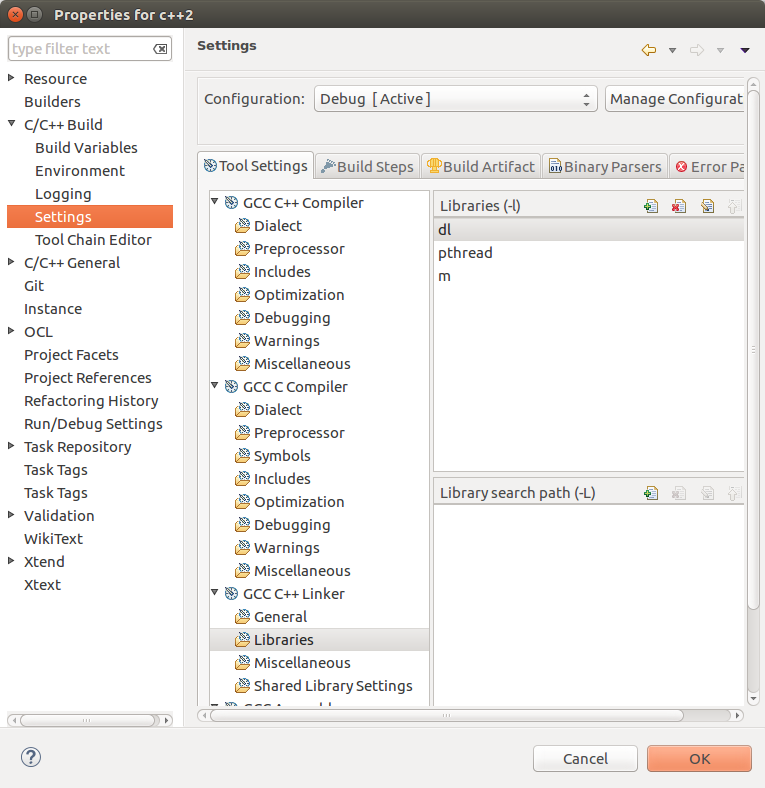
\includegraphics[width=\textwidth]{images/image12.png}
\end{center}
\caption{}
\label{fig:image12}
\end{figure}

Note that the code provided by default in the \textit{c++2} project
from the Git repository does not compile by itself. TTool must first be executed
to generate the classes specific to the system being simulated. Once this is
done, the simulator can be compiled and executed from CDT for the desired build
configuration.

\subsubsection{Launching the Simulator}

Like for JDT, the launch of C++ applications can be specified using the launch
configurations dialog as introduced in section~\ref{sec:launch}. One launch
configuration is provided for each build configuration and named
\textit{c++2 TTool} and \textit{c++2 Debug}.

\subsubsection{Using the Debugger}

The CDT debugger is very similar to the JDT debugger. However to be able to use
it only the \textit{c++2 Debug} launch configuration should be used and
triggered from the \textit{Debug As} button. By default, the program execution
will automatically stop at the first instruction of the program. This behavior
can be changed by editing the debug launch configuration.


\section{Coding Instructions}
Here are gather all tricks on how TTool source codes are organized, and what function is coded where, and also how to extend TTool, e.g. adding a new diagram.

\subsection{General rules}

\begin{itemize}
\item Indentations should use 4 spaces for each indentation level.
\item Do ensure your file is correctly indented before committing/pushing it
\end{itemize}


\subsection{How to output debug information}
Do as follows:
\begin{lstlisting}
TraceManager.addDev("blah blah blah");
\end{lstlisting}
Then, start TTool with the 
\begin{verbatim}
 -debug
\end{verbatim}
option.
Thus, to print information, never use:
\begin{lstlisting}
System.out.println("blah blah blah");
\end{lstlisting}
or similar ways of doing.

\subsection{Code organization}
Sources of "TTool" are located in "src/"\\
Basically, all graphical-related elements are put in "ui". All other subdirectories of "src" are used to code generic functions ("myutil") or non graphical languages and model transformation. for example, in "avatartranslator/" you find all classes related to the internal avatar language, and all transformations from the internal avatar to other languages (e.g. to UPPAAL) are in subdirectories of "avatartranslator/touppaal"
\subsubsection{User Interface directories}
Main classes are located directly in "src/ui". Subdirectories of "ui/" are mostly used for diagrams (one diagram per subdirectory, e.g. avatarbd for the Avatar Block Diagram). Other subdirectories are explained in the following table.
\begin{tabular}{l|c}
subdirectory&Explanation\\
\hline
file&Contains the definition of file extensions used by TTool\\
graph&AUT graph definition, and how to display an AUT graph\\
interactivesimulation&Graphical part of Diplodocus model simulation\\
tree&Ttree located in the upper left part of the main TTool Window.\\
window&Sub-windows: dialogs, frames, etc.
\end{tabular}

\subsection{Structure of the User Interface}
Actions of the main user interface are defined in "TGUIActions.java". The corresponding method which is called when an action occurs is defined in "ActionPerformer.java".

\subsection{Structure of a diagram}


\subsection{Error management}
The tree on the left contains a part dedicated to errors and warnings. The list of errors/warnings that is displayed by the tree is handled in GTURTLEModeling.java with:
\begin{lstlisting}
private List<CheckingError> checkingErrors;
private List<CheckingError> warnings;
\end{lstlisting}

\section{Testing}

It is planned to develop more and more tests for TTool in order to improve the
product quality. Test architectures are defined for each languages used to
develop TTool; Java and C++.

The testing code of TTool is located under the \textit{test} directory of the TTool
repository. A structure where a subdirectory is created for each
component of TTool to be tested (e.g.: Avatar, Diplodocus, shared utility
functions, etc.) is recommended. Each subdirectory can be further subdivided for
the different subcomponents of the component. For example, the Diplodocus component can be
further divided into its simulator and GUI components, which are not tested
under the same test environement and framework due to the different languages
used to develop these components.

A recommended practice consists of naming the folders containing the classes
with the same name of root package of the provided classes such as
$fr.tpt.ttool.tests.component\_name$, where $component\_name$ is the name of the
component of TTool being tested.

\subsection{Java}

The TTool Java code is tested using JUnit (\url{http://junit.org/}), which is a
unit test framework allowing to write, execute and display the results of
repeatable tests.

\subsubsection{Coding the Tests}

JUnit builds on a set of assertions for evaluating test results
and a set of annotations for qualifying test classes and methods. A test unit in
JUnit consists of a Java class grouping a set of test cases implemented as
methods of the class and identified with the $@Test$ annotation.
Other methods of the class to be executed only once before or after the
execution of all test cases of the classe can be identified from the annotations
$@BeforeClass$ and $@AfterClass$. Methods to be executed before or after each
test case is executed can be identified from the annotations $@Before$ and
$@After$.

When using the Eclipse IDE, test classes can be automatically generated for a
given class to be tested and will includ annotated methods for the selected
methods of the class to be tested.

See folder $test/fr.tpt.ttool.tests.util$ of the TTool source code repository
for an examp;e test class $TestRshClient$ providing test cases for the TTool
utility class $RshClient$ used for client-server remote communications.

\subsubsection{Executing the Tests}

\textbf{\emph{Using the JUnit Execution API}}

A JUnit test class can be executed automatically by passing
it to a JUnit test runner service that will take care of calling the appropriate
methods in the appropriate order to execute the tests, and return a test result
object that can be inspected to determine the succes or failure of the test
cases and provide more details in case of failure. An example code snippet is
showned below:

\begin{verbatim}
import org.junit.runner.JUnitCore;
import org.junit.runner.Result;
import org.junit.runner.notification.Failure;
import fr.tpt.ttool.tests.util.remote.TestRshClient;

public class TToolUtilTestsRunner  {

    public static void main(String[] args) {
        Result result = JUnitCore.runClasses(TestRshClient.class);

        for ( final Failure failure : result.getFailures() ) { 
            System.err.println( "Test failed : " + failure.toString() );
        }
 		
        if ( result.wasSuccessful() ) {
            System.out.println( "All tests passed." );
        }
        else {
            System.err.println( "Some of the tests failed!" );
        }
 
        System.exit( 0 );
    }
}
\end{verbatim}

\textbf{\emph{Within the Eclipse IDE}}

Like for C++ and Java applications, JUnit launch configurations can be defined
in Eclipse as shown in figure~\ref{fig:image13}. This configuration will execute all unit tests
for class \textit{RSHClient} and display within the IDE a view of the status of
the tests (passed of failed) as shown in figure~\ref{fig:image14}.

\begin{figure}[H]
\begin{center}
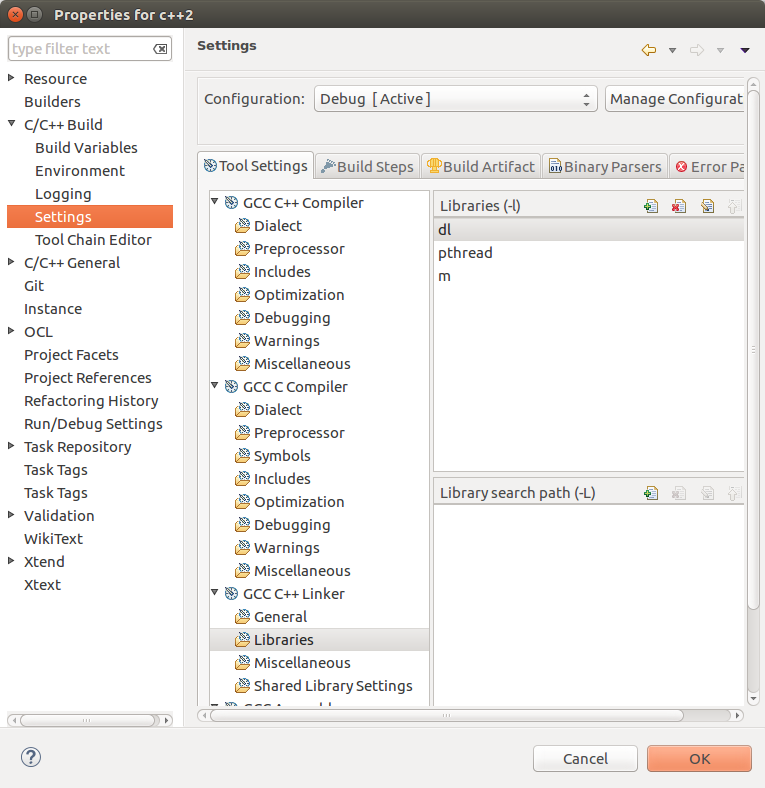
\includegraphics[width=\textwidth]{images/image13.png}
\end{center}
\caption{}
\label{fig:image13}
\end{figure}

\begin{figure}[H]
\begin{center}
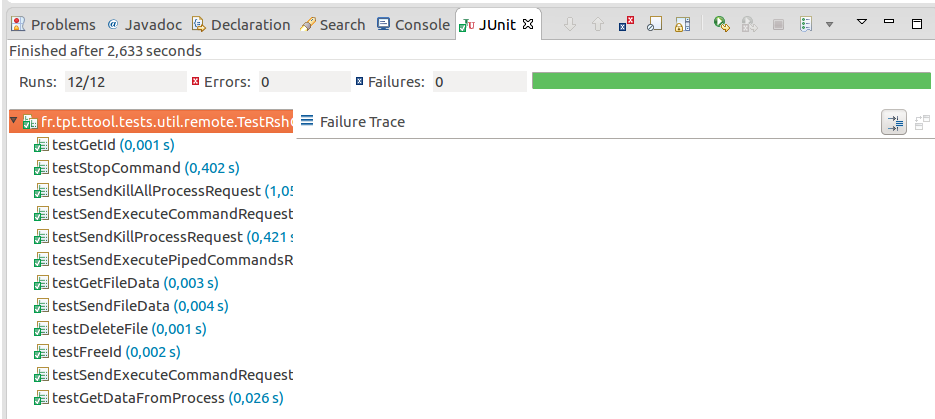
\includegraphics[width=\textwidth]{images/image14.png}
\end{center}
\caption{}
\label{fig:image14}
\end{figure}

\subsection{C++}

TODO

\section{Building}

\subsection{Compiling and Packaging}

First obtain the TTool repository from the Gitlab server as explaines in section
\ref{sec:scm}. From a Linux shell, CD to the root TTool directory and execute
\emph{make all} to compile the code. If the compilation fails with the following error:
``unmappable character for encoding ASCII'', you need to do:

\emph{export JAVA\_TOOL\_OPTIONS=-Dfile.encoding=UTF8} \\

For generating a release, execute \emph{make release}.

\subsection{Automated Tests}
TODO

\section{Installing}
TODO

\end{document}
